%%%%%%%%%%%%%%%%%%%%%%%%%%%%%%%%%%%%%%%%%
% Beamer Presentation
% LaTeX Template

\documentclass{beamer}
\mode<presentation> {
\usetheme{Warsaw}
}

\usepackage{multicol}
\usepackage[russian]{babel}
\usepackage{graphicx} 
\usepackage{hyperref}

\title[Introduction to Python]{Web scraping} 
\author{Sugarkhuu Radnaa} 
\institute[]
{
Py4Econ in Ulaanbaatar \\ 
\medskip
\textit{py4econ@gmail.com} 
}
\date{18 December, 2021}  % \today

\begin{document}

\begin{frame}
\titlepage % Print the title page as the first slide
\end{frame}

\begin{frame}
    \frametitle{Week 6: Learning objectives}
    \begin{enumerate}
        \item Setup selenium and chromedriver on your machine
        \item Extract data from websites!
    \end{enumerate}
\end{frame}

%------------------------------------------------
\section{Data types and structures} 
%------------------------------------------------

\begin{frame}
    \frametitle{Why Selenium?}

    There are many, many automation testing tools. We will use Selenium because it does pretty much all that I needed. There is no reason
    that the others are better at different tasks. Do let me know if you know or find such cases. 

    \begin{itemize}
        \item Selenium
        \item Beautiful Soup
        \item Scrapy
        \item Urllib
        \item MechanicalSoup
        \item LXML
        \item Python Requests
    \end{itemize}
\end{frame}


\begin{frame}
\frametitle{Chromedriver is needed}
    \begin{itemize}
        \item To control Chrome through Python
        \item Chromedriver should be in your system path
            \begin{itemize}
                \item Know your chrome version: \url{chrome://settings/help}
                \item Download a compatible chromedriver from: \url{https://chromedriver.chromium.org/downloads}
                \item Unzip and place it somewhere easy to access like: \url{C:\\Users\\sugarkhuu\\chromedriver\_win32}
            \end{itemize}
    \end{itemize}
\end{frame}

\begin{frame}
    \frametitle{Chrome Inspect (Ctrl + Shift + I)}
        \begin{itemize}
            \item Elements
        \end{itemize}
\centering
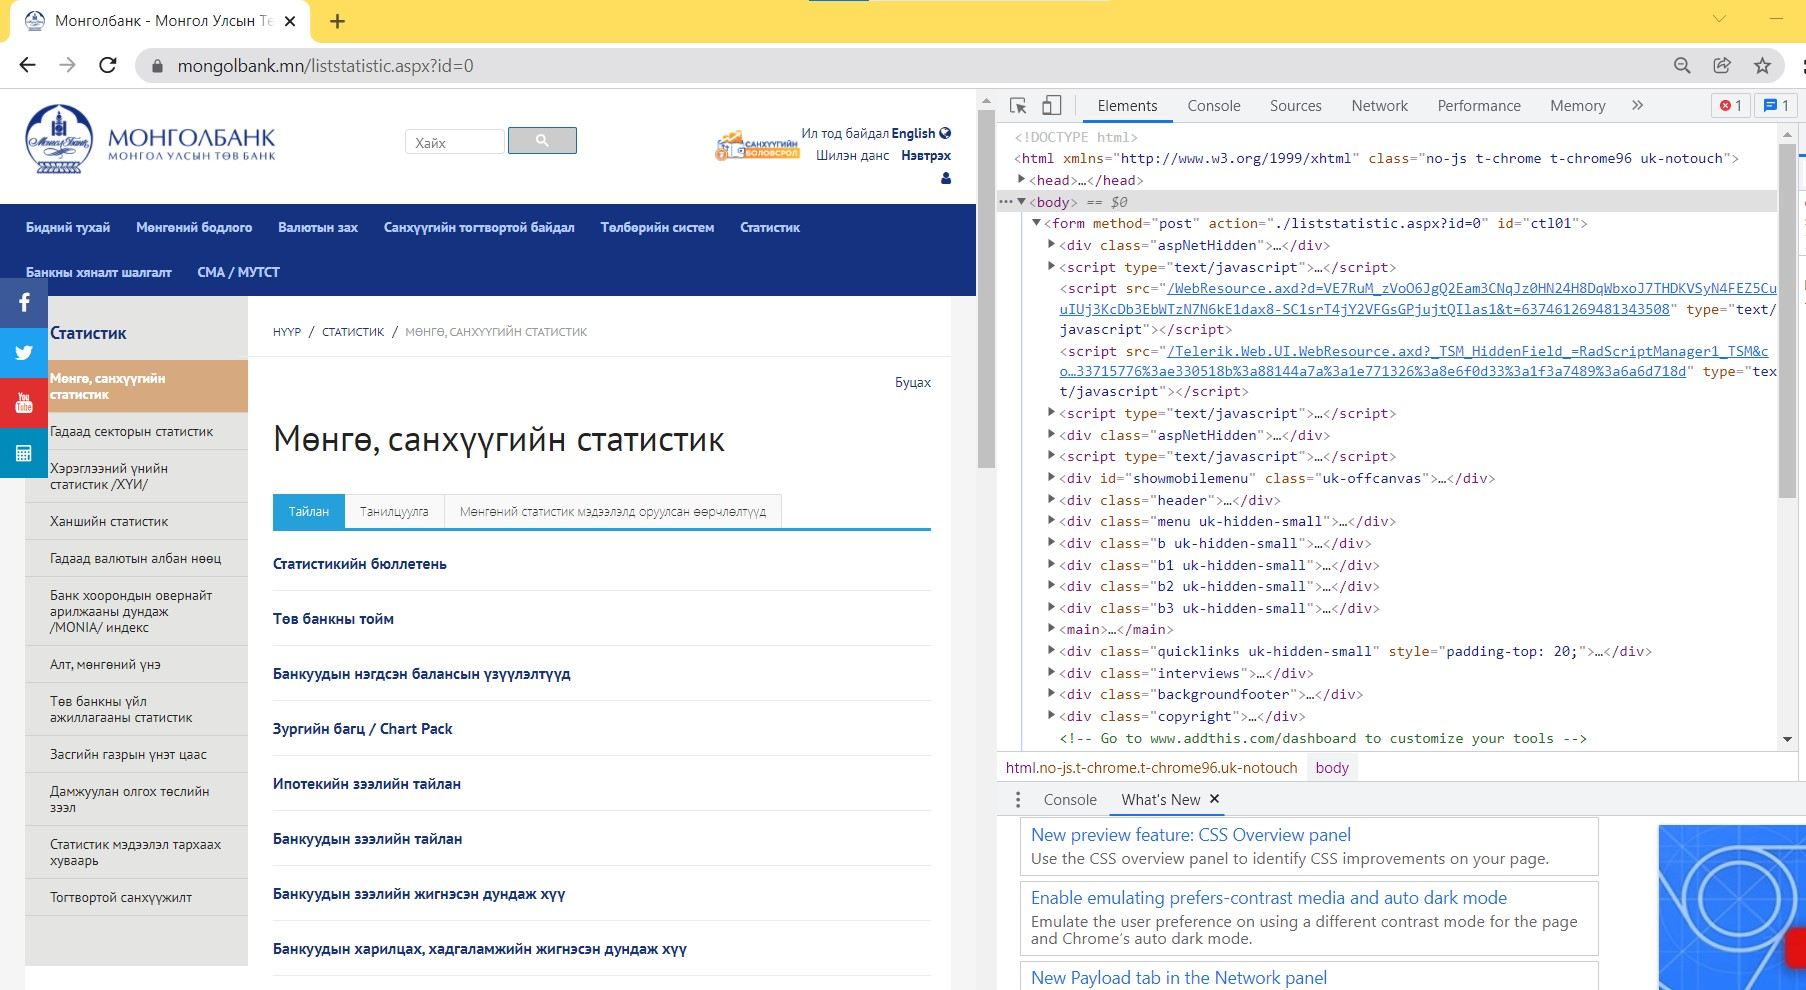
\includegraphics[scale=0.25]{figures/bom.jpg}
\end{frame}

\begin{frame}
\frametitle{HTML elements}
    \begin{itemize}
        \item Tags (html, head, body, a, nav, title, div, h1, h3, p, button, ...)
        \item Attributes (id, class, text, link, name, type, href, ...)
    \end{itemize}
\centering
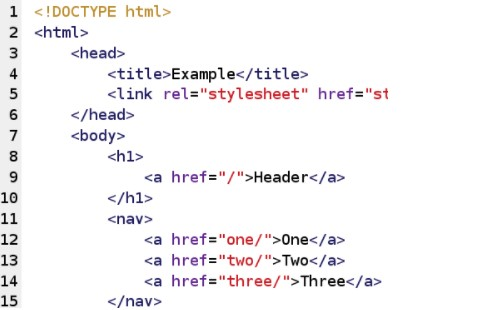
\includegraphics[scale=0.5]{figures/html.jpg}

\begin{flushleft}
    \textbf{HTML + CSS + Javascript = Web} \\
    See basics of HTML - \url{https://www.w3schools.com/html/html_paragraphs.asp}    
\end{flushleft}

\end{frame}

\begin{frame}
    \frametitle{Locating HTML elements}
    \begin{itemize}
        \item id
        \item name
        \item xpath (full xpath)
        \item class name
        \item text (with contains)
        \item tag
        \item css selector
        \item link\_text
    \end{itemize}
\end{frame}

\begin{frame}
    \frametitle{Navigating}
    \begin{itemize}
        \item send\_keys
        \item clear
        \item click
        \item get
        \item forward
        \item back
        \item text
        \item switch\_to\_window
    \end{itemize}
\end{frame}

%------------------------------------------------
\section{Homework} 
%------------------------------------------------

\begin{frame}
    \frametitle{No Homework, but Project!}
    
\begin{flushleft}
    Онлайн худалдааны ямар нэг платформ сонгон нэг төрлийн бүтээгдэхүүний хувьд
    нэмэлт бүтээгдэхүүн орж ирэхэд тодорхой имейл хаяг бүхий хэрэглэгчид рүү 
    имейл илгээдэг байх код бичнэ үү. 

    \begin{enumerate}
        \item Шалгах давтамжийг сонгох – Task scheduler (cron job), next week
        \item Хуучин дата хадгалах – csv, pickle, json
        \item Имейл нь шинэ бүтээгдэхүүний мэдээллийг агуулах хэрэгтэй – Email, next week
    \end{enumerate}

    \tiny
Дараах үйлдлүүд хийгдэх болов уу
    \begin{enumerate}
        \item Ямар нэг бүтээгдэхүүн сонгоно. Хөргөгч, угаалгын машин г.м. 
        \item Тухайн төрлийн бүх бүтээгдэхүүний мэдээллийг түүнэ. 
        \item Түүсэн мэдээллээ файл эсвэл өгөгдлийн санд хадгална.
        \item Тогтоосон хугацааны дараа вэбсайтаа дахин шалган, мэдээллийг түүнэ. 
        \item Шинэ мэдээллийг өмнөх хадгалсан мэдээлэлтэй харьцуулна. 
        \item Хоёр мэдээлэл ялгаагүй бол зогсоно. 
        \item Хоёр мэдээлэл ялгаатай байвал шинээр орж ирсэн бүтээгдэхүүнүүдийг ялгаж авна. 
        \item Шинэ бүтээгдэхүүний мэдээлэл бүхий имейл загвар үүсгэнэ. 
        \item Үүсгэсэн имейл загвараа имейлийн жагсаалт руу илгээнэ. 
        \item Шинэ болон хуучин датаг нэгтгэн, давхардлыг арилгаад хадгална. 
        \item Тогтсон хугацааны дараа дахин вэбсайтаа шалгана ...
    \end{enumerate}

\end{flushleft}
\end{frame}

\begin{frame}
\Huge{\centerline{Thank you!}}
\end{frame}

%----------------------------------------------------------------------------------------

\end{document} 